\documentclass[10pt]{article}
\usepackage{tikz}
\usetikzlibrary{arrows,decorations.pathmorphing,backgrounds,fit,positioning,shapes.symbols,chains}
\usetikzlibrary{decorations.pathreplacing}
\begin{document}
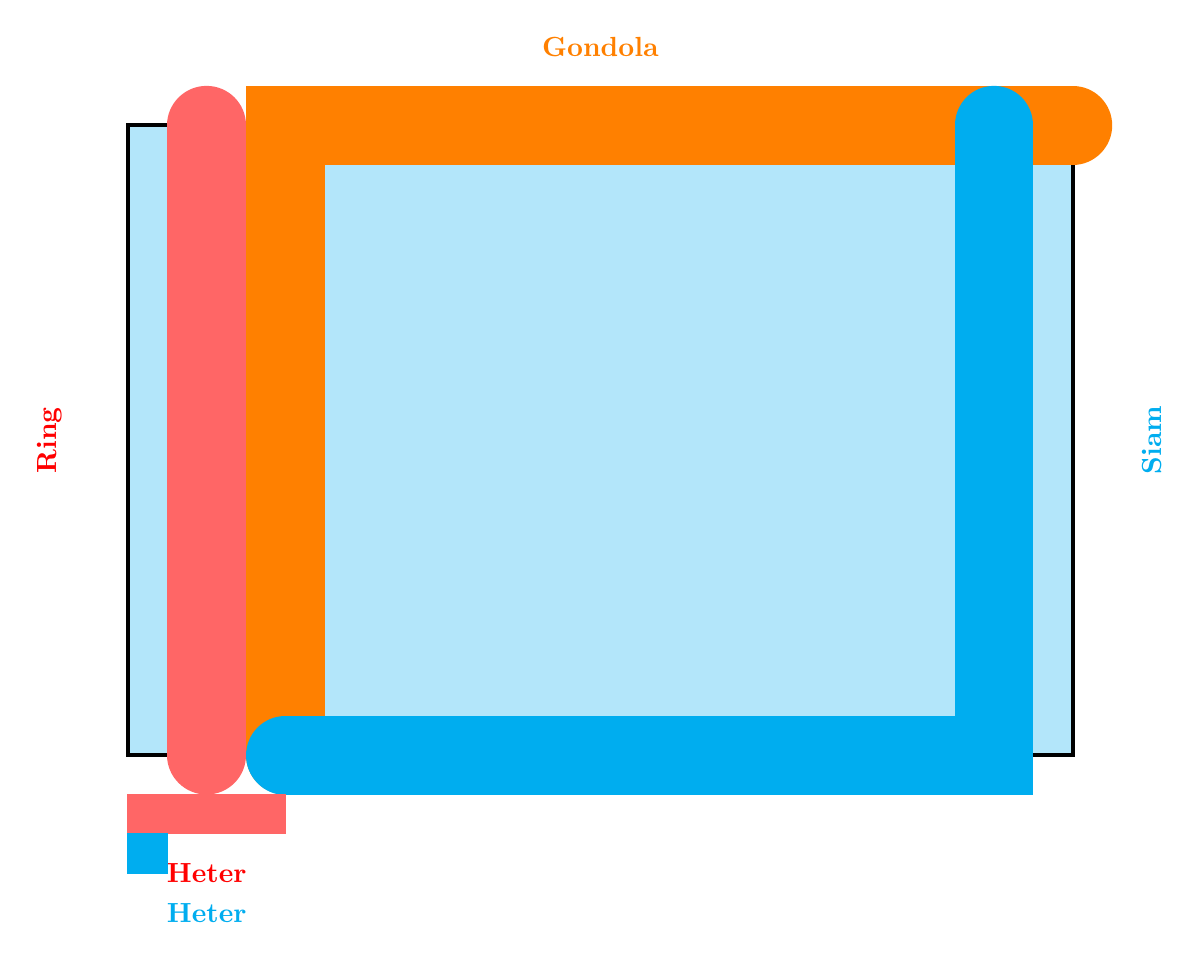
\begin{tikzpicture}
\draw[black, ultra thick,fill=cyan!30] (0,0) rectangle (12,8);
\draw[red!60, line width=1cm, line cap=round] (1,0) -- (1,8);
\draw[orange, line width=1cm, line cap=round] (2,0) -- (2,8) -- (12,8);
\draw[cyan, line width=1cm, line cap=round] (2,0) -- (11,0) -- (11,8);
\node[rotate=90] at (-1,4) {\textcolor{red}{\textbf{Ring}}};
\node[rotate=90] at (13,4) {\textcolor{cyan}{\textbf{Siam}}};
\node at (6,9) {\textcolor{orange}{\textbf{Gondola}}};
\draw[red!60,fill=red!60] (0,-1) rectangle (2,-0.5);
\node at (1,-1.5) {\textcolor{red}{\textbf{Heter}}};
\draw[orange,fill=orange] (0,-1.5) rectangle (0.5,-1);
\draw[cyan,fill=cyan] (0,-1.5) rectangle (0.5,-1);
\node at (1,-2) {\textcolor{cyan}{\textbf{Heter}}};
\end{tikzpicture}

\end{document}